\documentclass{article}

% --- Optimización de Codificación y Lenguaje ---
\usepackage[T1]{fontenc}
\usepackage[utf8]{inputenc}
\usepackage[spanish]{babel}

% --- Configuración de Página ---
\usepackage[letterpaper,top=2cm,bottom=2cm,left=3cm,right=3cm,marginparwidth=1.75cm]{geometry}

% --- Paquetes de Matemática y Gráficos ---
\usepackage{amsmath}
\usepackage{amssymb}
\usepackage{graphicx}
\usepackage{titling}
\usepackage[table]{xcolor} % Consolidación de colortbl y xcolor
\usepackage{etoolbox}
\usepackage{setspace}

\onehalfspacing % -- Interlineado

% --- Lógica de Estructura ---
\pretocmd{\section}{\clearpage}{}{}

% --- Configuración de Hipervínculos (Posicionamiento Crítico al Final) ---
\usepackage[colorlinks=true, allcolors=blue]{hyperref}

\title{Matemática Discreta}
\author{Angel Castiglia}
\date{Marzo, 2026}

\begin{document}
\maketitle

% --- Estructura de Navegación ---
\tableofcontents
\newpage

\section{Introducción}
\label{sec:introduccion}

La Matemática Discreta es la rama de las matemáticas que se ocupa del estudio de estructuras cuyos elementos pueden contarse uno por uno, es decir, que son separables o discontinuas. A diferencia del cálculo o el análisis matemático, que se centran en el "continuo" (números reales, curvas suaves, cambio infinitesimal), la matemática discreta opera sobre conjuntos finitos o infinitos numerables (como los números enteros).

\subsection{Aislamiento Algebraico}
\label{sec:aislamiento-algebraico}

Una estructura matemática se clasifica como discreta cuando sus elementos constitutivos existen en un estado de separación fundamental, desprovistos de una densidad continua intercalada. En marcado contraste con los dominios del continuo (como los números reales, gobernados por el análisis infinitesimal y la infinitud de puntos intermedios), los espacios discretos como los números enteros ($\mathbb{Z}$) se caracterizan por el aislamiento algebraico: cada elemento está flanqueado por un sucesor y un predecesor inmediatos y discretos, suprimiendo cualquier posibilidad de subdivisión infinita o acumulación puntual.

\begin{itemize}
\item En el conjunto de los enteros ($\mathbb{Z}$): Si tomamos el número 5, el intervalo abierto $(4, 6)$ solo contiene un elemento del conjunto: el propio 5. Esta separación garantiza que no haya "puntos de acumulación".
\item Contraste con el Continuo ($\mathbb{R}$): En los números reales, cualquier intervalo, por pequeño que sea, contiene una cantidad infinita de puntos. Esto es lo que permite el cálculo infinitesimal, pero hace imposible la enumeración uno por uno que define a la matemática discreta.
\end{itemize}

\subsection{Áreas de Estudio Fundamentales}
\label{sec:areas-estudio}

La matemática discreta no es una sola disciplina, sino un conjunto de teorías interconectadas:
\begin{itemize}
    \item Lógica y Álgebra de Boole: El fundamento de los circuitos digitales y la programación.
    \item Teoría de Conjuntos y Relaciones: El estudio de colecciones de objetos y cómo se vinculan entre sí.
    \item Teoría de Grafos: El modelado de relaciones entre objetos.
    \item Combinatoria: El arte de contar. Se encarga de determinar el número de formas posibles en que se pueden organizar o seleccionar elementos de un conjunto (permutaciones, combinaciones).
    \item Teoría de Números: El estudio de las propiedades de los números enteros, particularmente los números primos, lo cual es la base de la criptografía moderna (como el algoritmo RSA).
\end{itemize}

\subsection{El Lenguaje de la Computación}
\label{sec:lenguaje-computacion}

Su importancia radica en que las computadoras son, por naturaleza, máquinas discretas: procesan información en pasos finitos y almacenan datos en unidades separadas (bits).

\section{Números Naturales}
\label{sec:numeros-naturales}

\subsection{Definición de los Números Naturales} 
\label{sec:definicion-numeros-naturales}

Sea $S \subseteq \mathbb{N}$ un conjunto tal que el número $1$ pertenece a $S$ y para cada $n$ $\in$ $S$ se tiene que $n+1$ también pertenece a $S$. Entonces $S$ es el conjunto de los números naturales.

\bigskip

Sea $S \subseteq \mathbb{N}$ tal que:
\begin{enumerate}
    \item $1 \in S$
    \item $\forall n \in S \implies (n+1) \in S$
\end{enumerate}
Entonces $S = \mathbb{N}$

\subsection{Inducción Matemática y Principio del Buen Orden}
\label{sec:induccion-buen-orden}

El Principio de Inducción Matemática y el Principio del Buen Orden son dos conceptos estructurales profundos que sustentan la teoría de números y las matemáticas discretas. Ambos principios rigen el comportamiento y la fundamentación formal de los conjuntos de números enteros y naturales. Matemáticamente, el Principio de Inducción y el Principio del Buen Orden son lógicamente equivalentes. Esto implica que, dentro del desarrollo axiomático, cualquiera de ellos puede tomarse como axioma inicial para demostrar la veracidad de los otros dos como teoremas consecuentes.

\subsection{Inducción Matemática}
\label{sec:induccion-matematica}

La inducción es el proceso de obtener un resultado general a partir del análisis de casos particulares. La inducción matemática es un método de demostración utilizado para probar que una propiedad o proposición $P(n)$ es verdadera para todos los valores enteros $n$ que son mayores o iguales a un valor inicial dado. A pesar de compartir nombre con la inducción empleada en las ciencias naturales empíricas, la inducción matemática es un proceso de razonamiento estrictamente deductivo. La inducción matemática constituye la herramienta y estructura matemática principal para comprobar suposiciones teóricas acerca de secuencias, series y procesos que ocurren repetidamente bajo patrones definidos.

\bigskip

Tipos de inducción:

\begin{itemize}
    \item Clásica, Débil o Primer Principio de Inducción 
    \item Fuerte, Inducción Completa o Segundo Principio de Inducción
    \item Inducción Estructural
    \item Inducción Transfinita
\end{itemize}

\subsubsection{Analogía del Efecto Dominó}
\label{sec:analogia-domino}

Para comprender el mecanismo lógico subyacente, la inducción suele visualizarse mediante la analogía de una fila infinita de fichas de dominó dispuestas verticalmente. Si se empuja y cae la primera ficha, y se garantiza que cada ficha está posicionada de tal manera que, al caer, derribará inexorablemente a la siguiente, se deduce con total certeza matemática que todas las fichas de la fila caerán.

\begin{figure}[htbp]
    \centering
    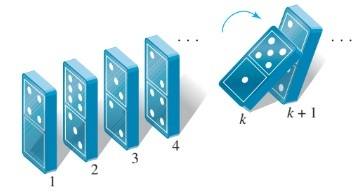
\includegraphics[width=0.4\textwidth]{imagenes/domino.jpg}
    \caption{Analogía del Efecto Dominó}
    \label{fig:domino-analogia}
\end{figure}

\begin{quote}
    \centering
    \noindent \textbf{Si la $k$-ésima ficha de dominó cae hacia atrás, también empuja a la $(k + 1)$-ésima ficha de dominó hacia atrás.}
\end{quote}

Para ver la conexión entre esta imagen y el principio de inducción matemática, sea $P(n)$ la frase “La enésima ficha de dominó cae hacia atrás”. Esta está dada para cada $k \geq 1$, si $P(k)$ es verdadera (la $k$-ésima ficha de dominó cae hacia atrás), entonces $P(k + 1)$ también es verdadera (la $(k + 1)$ ficha de dominó cae hacia atrás). También es debido a que $P(1)$ es verdadera (la primera ficha de dominó se cae hacia atrás). Así, con el principio de inducción matemática, $P(n)$ (la enésima ficha de dominó cae hacia atrás) es verdadera para cada entero $n \geq 1$.
\bigskip 

Si sabemos que una determinada afirmación es verdadera para algunos casos particulares, surge la pregunta. ¿Dicha afirmación sigue siendo verdadera para los infinitos números naturales restantes?
\bigskip 

Existen muchas afirmaciones que sólo son válidas para un número finito de casos y en consecuencia son falsas para un número infinito de situaciones. Sin embargo, podemos encontrar proposiciones (afirmaciones) que son verdaderas para todos los números naturales.
\bigskip

Analicemos los siguientes ejemplos: 
\noindent La proposición $p = n^2 \geq 1; \forall n \in \mathbb{N}$ es verdadera para todos los números naturales pero la proposición $q = n \geq 4; \forall n \in \mathbb{N}$ es falsa pues $\exists n \in \mathbb{N}$ tal que $n < 4$, como es el caso de $n = 1$.
\bigskip

La técnica de demostración por inducción matemática es utilizada para probar que proposiciones de la forma $\forall x:P(n)$ enunciadas sobre el conjunto de los números naturales son verdaderas, o sea si la proposición $p$ está dada para cada $n \in \mathbb{N}$ por una afirmación $p(n)$, probar que $p(n)$ es Verdadera para todo $n \in \mathbb{N}$.

\subsubsection{Demostración por Inducción Matemática: Pasos}
\label{sec:pasos-induccion-matematica}
La demostración por la técnica de Inducción Matemática consiste en dos pasos:
\begin{itemize}
\item \textbf{Paso Base:} para n = primer elemento del conjunto considerado. Se demuestra la validez de la proposición $p$ evaluada para el primer elemento del conjunto. Puede ser cualquier número natural dependiendo del punto de partida o condición inicial del problema que se está demostrando.

\item\textbf{Paso Inductivo:} 
Consiste en demostrar que la implicación $P(h) \to P(h + 1)$ es verdadera.
\end{itemize}
\bigskip

\noindent \textbf{Hipótesis y Tesis Inductivas}
\bigskip

\indent Se llama \textbf{Hipótesis inductiva} a \textbf{P(h)}, es decir la proposición o afirmación evaluada para \textbf{n=h}. Se asume que la hipótesis inductiva es Verdadera.
\bigskip

\indent Se llama \textbf{Tesis inductiva} a \textbf{P(h + 1)}, es decir la proposición o afirmación evaluada para \textbf{n=h+1}.

\subsubsection{Enunciado: Primer Principio de Inducción Matemática, Débil o Clásica}
\label{sec:enunciado-induccion-clasica}

Sea $P(n)$ una propiedad que se define para enteros $n$ y sea $a$ un entero fijo. Suponga que los siguientes dos enunciados son verdaderos:

\begin{enumerate}
    \item $P(a)$ es verdadera.
    \item Para todo entero $k \geq a$, si $P(k)$ es verdadera entonces $P(k + 1)$ es verdadera.
\end{enumerate}

Entonces, el enunciado para todo entero $n \geq a$, $P(n)$ es verdadero.

\subsubsection{Ejemplo: Suma de los \texorpdfstring{$n$}{n} Primeros Enteros}
\label{sec:ejemplo-suma-enteros}

\noindent Utilizar inducción matemática para demostrar que
\[
1 + 2 + \dots + n = \frac{n(n + 1)}{2} \text{ para todo entero } n \geq 1.
\]

\bigskip
\noindent \textbf{Solución por Inducción} \quad Para construir una demostración por inducción, primero debe identificar la propiedad $P(n)$. En este caso, $P(n)$ es la ecuación
\begin{center}
    \begin{tabular}{|c|}
        \hline
        \\
        $1 + 2 + \dots + n = \dfrac{n(n + 1)}{2}$ \\
        \\
        \hline
    \end{tabular} \quad { $\leftarrow$ la propiedad ($P(n)$)}
\end{center}

\bigskip
\textit{[Paso Básico]}

En el paso básico de la demostración, debe verificar que la propiedad es verdadera para $n = 1$, o, dicho de otro modo que $P(1)$ es verdadera. Ahora $P(1)$ se obtiene sustituyendo $1$ en lugar de $n$ en $P(n)$. El lado izquierdo de $P(1)$ es la suma de todos los enteros sucesivos empezando en 1 y terminando en 1. Este es exactamente 1. Así $P(1)$ es

\begin{center}
    \begin{tabular}{|c|}
        \hline
        \\
        $1 = \dfrac{1(1 + 1)}{2}$ \\
        \\
        \hline
    \end{tabular} \quad {$\leftarrow$ básico $P(1)$}
\end{center}

Por supuesto, esta ecuación es verdadera ya que el lado derecho es
\[
\frac{1(1 + 1)}{2} = \frac{1 \cdot 2}{2} = 1,
\]
que es igual al lado izquierdo.

\bigskip
\textit{[Paso Inductivo]}

En el paso inductivo, se supone que $P(k)$ es verdadera para un entero $k$ dado, pero elegido arbitrariamente con $k \geq 1$. \textit{Esta suposición es la hipótesis inductiva.} Entonces, debemos demostrar que $P(k + 1)$ es verdadera. ¿Qué son $P(k)$ y $P(k + 1)$? $P(k)$ se obtiene sustituyendo $k$ para todo $n$ en $P(n)$. Por tanto, $P(k)$ es

\begin{center}
    \begin{tabular}{|c|}
        \hline
        \\
        $1 + 2 + \dots + k = \dfrac{k(k + 1)}{2}$ \\
        \\
        \hline
    \end{tabular} \quad {$\leftarrow$ hipótesis inductiva ($P(k)$)}
\end{center}

\bigskip

Del mismo modo, $P(k + 1)$ se obtiene sustituyendo la cantidad $(k + 1)$ para todo $n$ que aparece en $P(n)$. Por tanto, $P(k + 1)$ es
\[
1 + 2 + \dots + (k + 1) = \frac{(k + 1)((k + 1) + 1)}{2},
\]
o, equivalente,

\begin{center}
    \begin{tabular}{|c|}
        \hline
        \\
        $1 + 2 + \dots + (k + 1) = \dfrac{(k + 1)(k + 2)}{2}$ \\
        \\
        \hline
    \end{tabular} \quad {$\leftarrow$ para mostrar ($P(k + 1)$)}
\end{center}

 \bigskip

La hipótesis inductiva es la suposición de que $P(k)$ es verdadera. ¿Cómo se puede usar esta suposición para demostrar que $P(k + 1)$ es verdadera? Una de las maneras más directas es utilizar la hipótesis inductiva junto con el álgebra para transformar por separado los lados izquierdo y derecho hasta que se vea que son iguales.

\bigskip

En este caso, el lado izquierdo de $P(k + 1)$ es
\[
1 + 2 + \dots + (k + 1) ,
\]
que es igual a
\[
(1 + 2 + \dots + k) + (k + 1) \quad 
\]

\bigskip

Pero sustituyendo la hipótesis inductiva,

\begin{align*}
    {(1 + 2 + \dots + k)} + (k + 1) &= {\frac{k(k + 1)}{2}} + (k + 1) \\
    &= \frac{k(k + 1)}{2} + \frac{2(k + 1)}{2} \\
    &= \frac{k^2 + k}{2} + \frac{2k + 2}{2} \\
    &= \frac{k^2 + 3k + 2}{2}
\end{align*}


\noindent El lado derecho de $P(k + 1)$ es $\dfrac{(k + 1)(k + 2)}{2}$. 

\noindent El lado izquierdo de $P(k + 1)$ es $\dfrac{k^2 + 3k + 2}{2}$.

\begin{center}
    \fbox{
        \begin{minipage}{0.3\textwidth}
            \centering            
            \[ \frac{(k + 1)(k + 2)}{2} = \frac{k^2 + 3k + 2}{2} \]             
        \end{minipage}
    }
\end{center}


Así, los dos lados de $P(k + 1)$ son iguales entre sí, por lo que la ecuación $P(k + 1)$ es verdadera.

\subsubsection{Ejemplo: Ciclo Invariante}
\label{sec:ejemplo-ciclo-invariante}

Un ciclo invariante es una afirmación acerca de variables de programa que es verdadera justo antes de que inicie la ejecución del ciclo y también después de cada iteración del ciclo. En particular, un ciclo invariante es verdadero cuando termina el ciclo, punto en el que el invariante nos dice algo acerca del estado de las variables. De manera ideal, esta afirmación dice que el ciclo produce el resultado esperado, es decir, que el ciclo es correcto. Por ejemplo, un ciclo invariante para un ciclo ``while'' (o mientras). Mediante la inducción matemática es posible probar que un invariante tiene el comportamiento deseado. El paso base demuestra que el invariante es verdadero antes de que la condición que controla el ciclo se pruebe la primera vez. El paso inductivo supone que el invariante es verdadero y después demuestra que si la condición que controla el ciclo es verdadera (de manera que el cuerpo del ciclo se ejecuta de nuevo), el invariante es verdadero después de ejecutar el cuerpo del ciclo. Como un ciclo itera un número finito de veces, la forma de la inducción matemática usada aquí demuestra que una secuencia finita de afirmaciones es verdadera. Se utiliza un invariante de ciclo para demostrar la corrección del siguiente algoritmo:

\begin{verbatim}
i = 1
fact = 1
while (i < n) {
    i = i + 1
    fact = fact * i
}
\end{verbatim}

Al finalizar la ejecución, se afirma que $fact = n!$. \bigskip


\noindent \textbf{Solución por Inducción}
Se demostrará que $fact = i!$ es un invariante para el ciclo. \bigskip

\textit{[Paso Básico]} 

Antes de la primera evaluación de la condición, $i = 1$ y $fact = 1$. Por definición, $1! = 1$, por lo tanto $fact = 1!$.

\bigskip

\textit{[Paso Inductivo]} 

Suponga que $fact = i!$ es verdadero. Si el ciclo se ejecuta, el nuevo valor de $i$ es $i + 1$ y el nuevo valor de $fact$ es:
    \[ fact \times (i + 1) = i! \times (i + 1) = (i + 1)! \]

Al finalizar el ciclo cuando $i = n$, la propiedad garantiza que $fact = n!$. \bigskip

\noindent \textbf{Prueba de Correctitud}

\begin{itemize}
    \item \textbf{Inicialización:} Antes de la primera iteración, $i = 1$ y $fact = 1$. Dado que $1! = 1$, la propiedad $fact = i!$ se cumple.
    \item \textbf{Mantenimiento:} Asumiendo que $fact = i!$ es verdadero al inicio de una iteración, tras incrementar $i$ en $1$ y actualizar $fact$ mediante el producto, obtenemos:
    \[
    fact_{nuevo} = fact \times (i + 1) = i! \times (i + 1) = (i + 1)!
    \]
    La propiedad se preserva para la siguiente iteración.
\end{itemize}

\subsubsection{Enunciado: Inducción Completa, Fuerte o Segundo Principio de Inducción}
\label{sec:induccion-fuerte}

Sea $P(n)$ una propiedad que se define para $n$ enteros y sean $a$ y $b$ enteros fijos con $a \leq b$. Suponga que los siguientes dos enunciados son verdaderos:

\begin{enumerate}
    \item $P(a), P(a + 1), \dots$ y $P(b)$ son todas verdaderas (\textbf{Paso básico.}).
    \item Para cualquier número entero $k \geq b$, si $P(i)$ es verdadera para todo entero $i$ de $a$ a $k$, entonces $P(k + 1)$ es verdadera (\textbf{Paso inductivo.}).
\end{enumerate}

Entonces el enunciado
\begin{equation*}
    \text{para todo entero } n \geq a, P(n),
\end{equation*}
es verdadero. (La suposición de que $P(i)$ es verdadera para todo entero $i$ de $a$ a $k$ se llama la \textbf{hipótesis inductiva}. Otra forma de indicar la hipótesis inductiva es decir, que $P(a), P(a + 1), \dots, P(k)$ son todas verdaderas.)
\bigskip

Se emplea fundamentalmente cuando la demostración de la proposición $P(k + 1)$ requiere asumir la verdad no solo de su predecesor inmediato, sino de múltiples o todos los casos anteriores.

\subsection{El Principio del Buen Orden}
\label{sec:principio-buen-orden}

El Principio del Buen Orden (también conocido como principio de buena ordenación) es un axioma fundamental en la teoría de números y las matemáticas discretas que establece una propiedad estructural esencial de los conjuntos numéricos discretos. Desde el punto de vista analítico y algebraico, este principio articula las siguientes áreas de estudio:

\begin{itemize}    
    \item \textbf{Equivalencia con la Inducción Matemática:} El principio del buen orden es lógicamente equivalente a las dos formas del principio de inducción matemática: la inducción clásica y la inducción fuerte. En el desarrollo axiomático de las matemáticas, cualquiera de estos principios puede asumirse como un axioma inicial para demostrar la veracidad de los otros como teoremas.
    \item \textbf{Fundamentación de Teoremas de Teoría de Números:} Este principio es el motor deductivo detrás de resultados clásicos de la aritmética. Se utiliza de manera directa para demostrar el \textit{Algoritmo de la División} (o teorema del cociente-residuo), garantizando que al dividir un entero existe un residuo mínimo no negativo. También es esencial en la demostración de la existencia del Máximo Común Divisor y proporciona las bases para demostrar el \textit{Teorema Fundamental de la Aritmética}.
    \item \textbf{Análisis y Terminación de Algoritmos:} En las ciencias de la computación, el principio del buen orden provee la justificación matemática de que ciertos procesos iterativos no entrarán en un ciclo infinito. Puesto que cualquier sucesión estrictamente decreciente de enteros no negativos debe ser forzosamente finita al estar obligada a alcanzar un mínimo, este axioma permite demostrar que algoritmos específicos terminarán su ejecución después de un número finito de pasos.
    \item \textbf{Generalización en la Teoría de Conjuntos:} En un marco de abstracción mayor, la teoría de conjuntos define que cualquier conjunto parcialmente ordenado está ``bien ordenado'' si cumple invariablemente que todo subconjunto no vacío posee un primer elemento. Bajo la axiomática de Zermelo-Fraenkel y el axioma de elección, el \textit{Teorema del Buen Orden} postula que absolutamente cualquier conjunto puede ser bien ordenado, lo cual da sustento a metodologías de demostración más avanzadas como la inducción transfinita.
\end{itemize}

\subsubsection{Enunciado del Principio}
\label{sec:enunciado-buen-orden}

\noindent El Principio del Buen Orden establece que cualquier subconjunto no vacío de los números naturales tiene un elemento mínimo.
\[
\boxed{\textit{Sea un conjunto } S \subseteq \mathbb{N} \land S \neq \emptyset \textit{ tal que } \exists m \in S \mid \forall n \in S, m \le n}
\]

\noindent En un subconjunto, siempre existirá un valor en él que sea menor o igual a todos los demás elementos de dicho subconjunto. Este principio indica que todo subconjunto de los números naturales está ''bien ordenado''.

\begin{figure}[htbp]
    \centering
    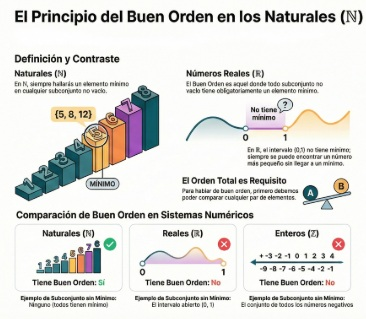
\includegraphics[width=0.4\textwidth]{imagenes/buen_orden.jpg}
    \caption{Esquema del Principio del Buen Orden}
    \label{fig:buen-orden-esquema}
\end{figure}
      
\subsubsection{Análisis del Principio del Buen Orden}
\label{sec:analisis-buen-orden}

\begin{itemize}
    \item \textbf{Premisa sobre el Conjunto $S$:} ``Sea $S \subseteq \mathbb{N}$'' establece que nuestro conjunto de interés, $S$, debe ser un subconjunto de los números naturales. $\mathbb{N}$ puede definirse como $\{1, 2, 3, \dots\}$ o $\{0, 1, 2, \dots\}$, según la convención, pero el principio se aplica a ambos.
    \item \textbf{Condición de Existencia:} ``$S \neq \emptyset \rightarrow \dots$'' es una implicación. La condición necesaria para que la conclusión se cumpla es que $S$ no sea el conjunto vacío. Es obvio que un conjunto sin elementos no puede tener un elemento mínimo.
    \item \textbf{La Existencia del Mínimo:} ``$\exists m \in S$ tal que ...'' nos garantiza la existencia de \textit{al menos un} elemento en $S$, al cual llamaremos $m$, que posee una propiedad única.
    \item \textbf{La Propiedad del Mínimo:} ``$m \leq n \forall n \in S$'' define qué es lo que hace de $m$ el elemento mínimo. Establece que $m$ es menor o igual a \textit{todos} los elementos $n$ que pertenezcan a $S$.
\end{itemize}

\textbf{Importancia:}

Este principio garantiza que no podemos tener una cadena descendente infinita de números naturales. Es decir, si empezamos a contar hacia atrás desde cualquier número natural, forzosamente nos detendremos en un punto (el mínimo), lo cual diferencia a $\mathbb{N}$ de conjuntos como los enteros ($\mathbb{Z}$) o los racionales positivos ($\mathbb{Q}^{+}$), donde siempre es posible encontrar un número menor.

\subsection{Implicancias entre PBO y PIM}
\label{sec:implicancias-entre-pbo-pim}

Es importante saber que no necesitamos tomar ambos principios como axiomas independientes; basta con suponer el PBO para probar la validez del PIM y viceversa. Esto demuestra que ambos principios son equivalentes (cada uno implica al otro) en el contexto de los números naturales.

\subsubsection{PBO Implica PIM}
\label{sec:pbo_implica_pim}

\noindent $PBO \implies PIM$

\bigskip

\noindent Demostración por contradicción
\begin{itemize}
\item Sea $S \neq \emptyset \land S \subset \mathbb{N}$ tal que
\begin{enumerate}
    \item $1 \in S$
    \item Si $k \in S$ entonces $(k+1) \in S$
\end{enumerate}
\item Suponemos que no se cumple PIM 

{$S \neq \mathbb{N}$ (contradicción)}

\item Si $S \neq \mathbb{N}$ consecuentemente $S^c \neq \emptyset$ (a) $S^c$ es un subconjunto de los $\mathbb{N}$ entonces admite el PBO.
\item $S^c$ tiene un elemento mínimo o primer elemento $t$

$t \in S^c \mid \forall m \in S^c \quad t \leq m$ (elemento mínimo) (b)

\item Si $t$ es el elemento mínimo de $S^c$, $t-1$ no puede estar en $S^c$

$t-1 \in S$

\item Por 1) y 2) sabemos que el elemento 1 y el siguiente $(k+1)$ están en $S$
\item Entonces $t-1+1 = t \in S \quad \}$ contradicción (c)
\item El elemento $t$ está en $S^c$ (b) y en $S$ (c)

Esta contradicción se debe a que supusimos que $S \neq \mathbb{N}$ en (a)

La contradicción entre (b) y (c) implica que

$S = \mathbb{N}$
\end{itemize}
\noindent Esto significa que PBO implica PIM.

\subsubsection{Análisis de la Implicación (PBO Implica PIM)}
\label{sec:analisis-pbo-pim}

\begin{itemize}
    \item \textbf{Establecimiento de las Premisas Axiomáticas:} Se define un conjunto $S$ que cumple estrictamente con las dos condiciones fundamentales de la inducción matemática: contiene al elemento $1$ (caso base), y si contiene a un elemento $k$, obligatoriamente contiene a su sucesor $k+1$ (paso inductivo). El objetivo natural sería concluir que $S = \mathbb{N}$.
    \item \textbf{Suposición para la Reducción al Absurdo:} La estrategia por contradicción exige suponer temporalmente que la conclusión deseada es falsa. Por lo tanto, se asume que $S \neq \mathbb{N}$, lo que lógicamente implica que la afirmación del PIM no se sostiene para este conjunto.
    \item \textbf{Invocación del Principio del Buen Orden (PBO):} Si $S$ no abarca todos los números naturales, su complemento relativo respecto a los naturales, denotado como $S^c$ (los elementos de $\mathbb{N}$ que no están en $S$), no es un conjunto vacío ($S^c \neq \emptyset$). Al ser $S^c$ un subconjunto no vacío de $\mathbb{N}$ se le aplica directamente el PBO, garantizando la existencia de un elemento mínimo absoluto dentro de ese complemento. A este elemento mínimo se le denomina $t$.
    \item \textbf{Construcción de la Paradoja Lógica:} Dado que $t$ es el elemento más pequeño que \textit{no pertenece} a $S$, su predecesor inmediato, $t-1$, no puede pertenecer al complemento $S^c$. Por la ley del tercero excluido, si $t-1$ es un número natural (asumiendo $t > 1$) y no está en $S^c$, obligatoriamente $t-1 \in S$. Al invocar la segunda premisa inicial (el paso inductivo): si un elemento pertenece a $S$, su sucesor también debe pertenecer. El sucesor de $t-1$ es precisamente $t$. Por aplicación estricta de la premisa, $t$ debe pertenecer a $S$.
    \item \textbf{Resolución Analítica y Conclusión:} Se ha derivado deductivamente que el elemento $t$ pertenece a $S^c$ (por definición del PBO) y, simultáneamente, $t$ pertenece a $S$ (por la premisa inductiva). Esto viola el Principio de No Contradicción formulado en la lógica aristotélica. La falacia lógicamente debe originarse en la premisa no demostrada: la suposición inicial de que $S \neq \mathbb{N}$ en (a). Al refutar esta suposición, queda demostrado indudablemente que $S = \mathbb{N}$. Así, asumir el PBO obliga a que el PIM sea verdadero.
\end{itemize}

\subsubsection{PIM Implica PBO}
\label{sec:pim_implica_pbo}

\noindent \textbf{Demostración} \\
\noindent Sea $A \subseteq \mathbb{N}$ con $A \neq \emptyset$ \\
\indent $\cdot$ \textbf{Caso 1:} $A$ tiene elemento mínimo. \\
\indent $\cdot$ \textbf{Caso 2:} $A$ no tiene elemento mínimo. \\
\noindent Consideremos la propiedad $P(m) :=$ ``los naturales del $1$ al $m$ no están en $A$''. \\
\noindent Sea $B = \{m \in \mathbb{N} \mid P(m) \text{ se cumple}\}$. Entonces:

\begin{enumerate}
    \item \textbf{$1 \in B$} \\
    Notemos que si $1 \in A \Rightarrow 1$ es elemento mínimo \textit{(Contradicción)}. \\
    $\therefore 1 \notin A$ y entonces $P(1)$ se cumple y $1 \in B$.
    \item \textbf{$n \in B \Rightarrow n+1 \in B$} \\
    Supongamos que $n \in B \Rightarrow P(n)$ se cumple $\Rightarrow$ los naturales de $1$ a $n$ no están en $A$. \\
    $\Rightarrow n+1 \notin A$, pues si $n+1 \in A$ pero $1, 2, \dots, n \notin A$, tendríamos que $n+1$ es un mínimo de $A$. \\
    $\Rightarrow$ los naturales entre $1$ y $n+1$ no están en $A \Rightarrow P(n+1)$ se cumple $\Rightarrow n+1 \in B$.
\end{enumerate}

\noindent Por PIM tenemos que $B = \mathbb{N}$. Notemos que si $m \in B \Rightarrow m \notin A$. Pero como $B = \mathbb{N}$ y $A \subseteq \mathbb{N} \Rightarrow A = \emptyset$ \textit{(Contradicción)}. \\
\noindent $\therefore A$ sí tiene elemento mínimo. 

\subsubsection{Análisis de la Implicación (PIM Implica PBO)}
\label{sec:analisis-pim-pbo}
\begin{itemize}    

\item \textbf{Estrategia Metodológica:} La estructura argumentativa se basa en una dicotomía y una posterior prueba por contradicción (\textit{reductio ad absurdum}). Se postula un conjunto $A \subseteq \mathbb{N}$ no vacío. El análisis se bifurca: el conjunto posee un mínimo, o carece de él. Al asumir la ausencia de mínimo, se inicia un proceso lógico diseñado para generar una incompatibilidad fundamental.
\item \textbf{El Predicado de Exclusión Acumulativa:} El eje de la demostración es la formulación de la propiedad $P(m)$: ``los naturales del $1$ al $m$ no están en $A$'', y la creación del conjunto auxiliar $B$. Esta técnica transforma una evaluación individual de elementos en una exclusión acumulativa, permitiendo que la Inducción Simple actúe con la robustez de la Inducción Fuerte.
\item \textbf{Evaluación del Caso Base:} Si el número $1$ perteneciera a $A$, actuaría como el mínimo absoluto, violando la premisa. Se deduce inexorablemente que $1 \notin A$, validando la pertenencia de $1$ al conjunto $B$.
\item \textbf{Transición Inductiva:} Bajo la hipótesis de que ningún natural hasta $n$ pertenece a $A$, la inclusión de $n+1$ en $A$ lo convertiría instantáneamente en el elemento mínimo. Para evitar esta contradicción con la premisa, $n+1$ debe quedar excluido de $A$, garantizando su ingreso al conjunto $B$.
\item \textbf{Conclusión por Reducción al Absurdo:} La inducción concluye que el conjunto excluyente $B$ abarca la totalidad de los naturales ($B = \mathbb{N}$). En consecuencia, el conjunto original $A$ carece de elementos ($A = \emptyset$), lo cual infringe directamente la hipótesis inicial ($A \neq \emptyset$). El colapso del Caso 2 demuestra que todo subconjunto no vacío de $\mathbb{N}$ debe poseer un elemento mínimo.
\end{itemize}


\section{Estructuras Algebraicas}
\label{sec:estructuras_algebraicas}


\subsection{Definición y Clasificación de Estructuras Algebraicas} 
\label{sec:definicion_clasificacion_estructuras_algebraicas}

\textbf{Las estructuras algebraicas} son sistemas matemáticos formales compuestos por uno o más conjuntos no vacíos, los cuales están dotados de una o varias operaciones (leyes de composición interna o externa) y, en ocasiones, de elementos singulares y relaciones, que satisfacen un conjunto riguroso de axiomas.

Formalmente, una estructura algebraica suele representarse mediante una n-tupla de la forma $(X, *, \circ, \dots, e, \dots)$, donde $X$ es el conjunto base o subyacente, $*$ y $\circ$ representan las operaciones binarias definidas sobre él, y $e$ denota posibles elementos singulares, como un neutro aditivo o multiplicativo.

El propósito fundamental al estudiar estas estructuras es generalizar y abstraer el comportamiento de los sistemas matemáticos habituales (como la aritmética básica de los números enteros o reales). Esta abstracción permite aplicar las mismas leyes lógicas y procedimentales a objetos de diversa naturaleza, tales como matrices, funciones, polinomios, conjuntos, proposiciones lógicas o transformaciones geométricas (como los grupos de simetría).

La clasificación axiomática de las estructuras algebraicas se realiza característicamente en función de la cantidad de operaciones que poseen y de las propiedades operativas que estas satisfacen:
 \bigskip

\textbf{Estructuras con una sola operación interna:}

\begin{itemize}
    \item Semigrupo
    \item Monoide
    \item Grupo
\end{itemize}

\textbf{Estructuras con dos operaciones internas:}

\begin{itemize}
    \item Anillo
    \item Cuerpo
    \item Álgebra de Boole
\end{itemize}

El rigor en la definición de estas estructuras provee las herramientas fundacionales para el análisis de algoritmos, la criptografía, la teoría de códigos y el diseño de circuitos lógicos.

Los \textbf{elementos singulares} son componentes específicos de un conjunto que desempeñan un rol único y distinguido bajo una ley de composición determinada. A diferencia de los elementos genéricos, los singulares poseen propiedades invariantes que definen el comportamiento global de la estructura.
Estos elementos se categorizan según su impacto en la operación destacando entre ellos: 
\begin{itemize}
\item Elemento neutro (o identidad)
\item Elemento Inverso
\item Elemento Absorbente
\item Elemento Involutivos
\item Regularidad o de Cancelacion
\end{itemize}

\textbf{Las leyes de composición} son las reglas fundamentales que permiten relacionar u operar los elementos de los conjuntos matemáticos. Se clasifican en:
\begin{itemize}
    \item Interna
    \item Externa
\end{itemize}

\subsection{Ley de Composición Interna} 
\label{sec:leyes_de_composicion_interna}

Una ley de composición interna es una operación definida sobre un conjunto no vacío que cumple con una regla fundamental: 
\bigskip

\textit{al tomar dos elementos cualquiera (par ordenado) de ese conjunto y operarlos entre sí, el resultado obtenido es siempre un elemento que también pertenece a ese mismo conjunto.}
\bigskip

Esto significa que la operación es un proceso cerrado: al tomar dos elementos cualesquiera del conjunto original y operarlos, el resultado jamás escapará de los límites de dicho conjunto. Esta propiedad de clausura o cerradura es el pilar fundamental para definir estructuras algebraicas más complejas como grupos, anillos o cuerpos.
\begin{itemize}
    \item Una \textbf{ley de composición interna} (u \textbf{operación binaria}) en un conjunto no vacío $A$ es efectivamente una función
    \[ \ast : A \times A \longrightarrow A. \]
    \item La notación $a \ast b$ representa el resultado de aplicar esa función al par $(a,b)$.
    \item La implicación $a \in A \land b \in A \implies a \ast b \in A$ expresa la \textbf{propiedad de clausura}, que es equivalente a que $\ast$ sea una función con codominio $A$.
\end{itemize}

\noindent El símbolo $\ast$ es un \textbf{operador genérico}: puede representar cualquier operación concreta (suma, multiplicación, composición, etc.), siempre que el resultado pertenezca al mismo conjunto $A$.
\bigskip

\noindent Ejemplo de tabla, que define una ley de composición interna en A
\bigskip

\noindent $A = \{a, b, c\}$ 
\bigskip

\noindent {$a \in A \land b \in A$} $\implies$ {$a \ast b \in A$} 
\bigskip

\noindent $(A, \ast)$ ¿Verifica la Ley de Composición Interna?

\begin{table}[htbp]
\centering
\begin{tabular}{|c|>{\columncolor{gray!25}}c|>{\columncolor{gray!25}}c|>{\columncolor{gray!25}}c|}
\hline
\rowcolor{gray!25}
\textbf{$\ast$} & \textbf{a} & \textbf{b} & \textbf{c} \\ \hline
\rowcolor{gray!25}
\textbf{a} & \cellcolor{gray!10}a & \cellcolor{gray!10}b & \cellcolor{gray!10}c \\ \hline
\rowcolor{gray!25}
\textbf{b} & \cellcolor{gray!10}b & \cellcolor{gray!10}c & \cellcolor{gray!10}a \\ \hline
\rowcolor{gray!25}
\textbf{c} & \cellcolor{gray!10}c & \cellcolor{gray!10}a & \cellcolor{gray!10}b \\ \hline
\end{tabular}
\end{table}
\noindent La operación $\ast$ es Ley de Composición Interna en A. 

\noindent Esta ley también es conocida como Ley de Cierre.

\subsubsection{Análisis de Ley de Composición Interna mediante Tablas de Cayley}
\bigskip

\begin{itemize}    
\item \textbf{Contexto Metodológico:} La imagen introduce una herramienta visual y combinatoria fundamental en el álgebra abstracta para conjuntos finitos: la Tabla de Cayley. Esta tabla permite definir exhaustivamente una operación binaria mostrando el resultado de operar cualquier par de elementos del conjunto.
\item \textbf{El Conjunto Finito:} Se define un conjunto $A = \{a, b, c\}$ con cardinalidad 3 ($|A| = 3$). Al ser finito y pequeño, la tabla es el método ideal para estudiar sus propiedades operacionales.
\item \textbf{Verificación Visual de la Ley de Composición Interna (Ley de Cierre):}
\begin{itemize} 
\item La pregunta central es si el par $(A, *)$ constituye un magma (una estructura algebraica dotada de una Ley de Composición Interna).
\item La condición formal $a \in A \land b \in A \implies a * b \in A$ se traduce visualmente en la tabla de la siguiente manera: se deben observar exclusivamente los resultados en el interior de la cuadrícula de $3 \times 3$ (excluyendo la fila y columna de los encabezados).
\item Al inspeccionar los 9 resultados interiores, notamos que todos pertenecen al conjunto original $\{a, b, c\}$. No aparece ningún elemento extraño o no definido (como un hipotético elemento $d$).
\item Esta inspección visual basta para afirmar categóricamente que la operación $*$ es cerrada, y por lo tanto, es una Ley de Composición Interna en el conjunto $A$.
\end{itemize}

\item \textbf{Terminología Equivalente:} En la literatura matemática, referirse a un conjunto como cerrado bajo una operación es exactamente lo mismo que decir que la operación es una Ley de Composición Interna o Ley de Cierre.
\end{itemize}
\bigskip

\noindent \textbf{Ejemplo de Ley de Composición Interna en A} 
\bigskip


\noindent $A = \{-1, 0, 1\} \quad (A, +)$
\bigskip

\noindent ¿Verifica la Ley de Composición Interna?

\begin{table}[htbp]
\centering
\begin{tabular}{|c|>{\columncolor{gray!30}}c|>{\columncolor{gray!30}}c|>{\columncolor{gray!30}}c|}
\hline
\rowcolor{gray!30}
\textbf{$+$} & \textbf{-1} & \textbf{0} & \textbf{1} \\ \hline
\rowcolor{gray!30}
\textbf{-1} & \cellcolor{gray!15}-2 & \cellcolor{white}-1 & \cellcolor{white}0 \\ \hline
\rowcolor{gray!30}
\textbf{0} & \cellcolor{white}-1 & \cellcolor{white}0 & \cellcolor{white}1 \\ \hline
\rowcolor{gray!30}
\textbf{1} & \cellcolor{white}0 & \cellcolor{white}1 & \cellcolor{gray!15}2 \\ \hline
\end{tabular}
\end{table}

\textit{ $+$ no es una ley de composición interna en A porque $-2$ y $2$ no pertenecen al conjunto A. }
\bigskip

\textbf{Otros Ejemplos}

\noindent \textbf{En los Números Naturales ($\mathbb{N}$):} La suma ($+$) es una ley de composición interna porque la suma de dos naturales es siempre un natural. Sin embargo, la resta ($-$) no lo es, ya que $3 - 5 = -2$ y -2 no pertenece al conjunto de los naturales.
\bigskip

\noindent \textbf{En los Números Reales ($\mathbb{R}$):} Las operaciones de adición ($+$) y multiplicación ($\cdot$) son ejemplos de leyes de composición interna, ya que la suma o el producto de dos números reales siempre resulta en un número real.
\bigskip

\textbf{Formalización}
\noindent Sea $G$ un conjunto no vacío, la operación $\ast$ se llama \textit{ley de composición interna} en $G$ si y solo si:

\[ a \in G \land b \in G \implies (a \ast b) \in G \]

\noindent $\ast$ es una ley de composición interna en $G$ si es una \textit{función} de la forma:

\begin{align*}
    \ast : G \times G &\to G \\
    (a;b) &\to a \ast b
\end{align*}

\bigskip

\noindent \textbf{Propiedad de Uniformidad}
\bigskip

La propiedad de uniformidad es la condición lógica que garantiza que el resultado de una operación es único y no presenta ambigüedades. Establece que al operar elementos idénticos se deben obtener resultados idénticos.
\bigskip

Si definimos una operación $\ast$ en un conjunto $G$, el principio de uniformidad se traduce en la propiedad de unicidad de la función. Formalmente, se expresa mediante la siguiente implicación:

\[ \forall a, b, c, d \in G : (a = c \land b = d) \implies a \ast b = c \ast d \]

Esto significa que si sustituimos los operandos por otros elementos idénticos (o expresiones equivalentes), el resultado final de la operación no debe alterarse. Es, en esencia, lo que permite el manejo de igualdades en el álgebra: si tenemos una ecuación $x = y$, podemos asegurar que $a \ast x = a \ast y$ gracias a este principio.

\subsection{Ley de Composición Externa} 
\label{sec:leyes_de_composicion_externa}

Una ley de composición externa es una operación matemática en la que, al tomar un elemento de un conjunto y operarlo con un elemento de otro conjunto distinto, el resultado obtenido pertenece a alguno de esos dos conjuntos. La característica fundamental de esta ley es que los conjuntos involucrados deben ser diferentes. A diferencia de la ley interna, donde los operandos y el resultado pertenecen al mismo conjunto, aquí se establece una relación de acción de un conjunto sobre otro.

\subsubsection{Ley de Composición Externa por Derecha o por Izquierda}

En el estudio de los sistemas algebraicos y la teoría de conjuntos, la distinción entre una ley de composición externa por la derecha o por la izquierda reside fundamentalmente en la posición que ocupa el operador (elemento del conjunto externo) respecto al operando (elemento del conjunto base). Esta distinción es crucial cuando la estructura no es necesariamente conmutativa o cuando el orden de aplicación define la interpretación semántica del sistema.
\bigskip
\begin{itemize}

\item \textbf{Ley de Composición Externa por la Derecha}
Sean $G$ y $H$ dos conjuntos no vacíos. Una operación $\ast$ es una ley de composición externa por la derecha si:
\[ a \in G \land b \in H \implies (a \ast b) \in G \]
\[ \ast : G \times H \to G \]

\item \textbf{Ley de Composición Externa por la Izquierda}
Sean $H$ y $G$ dos conjuntos no vacíos. Una operación $\ast$ es una ley de composición externa por la izquierda si:
\[ \alpha \in H \land a \in G \implies (\alpha \ast a) \in G \]
\[ \ast : H \times G \to G \]
\end{itemize}

\subsubsection{Análisis de Lateralidad}

\bigskip

A diferencia de las Leyes de Composición Interna, que operan estrictamente dentro del producto cartesiano de un único conjunto ($G \times G$), las Leyes de Composición Externa definen interacciones entre dos conjuntos distintos: un conjunto base $G$ y un conjunto de operadores $H$. La función establece un mapeo donde la aplicación de un elemento de $H$ sobre un elemento de $G$ proyecta el resultado inexorablemente de vuelta al conjunto base $G$.
\bigskip

\noindent \textbf{Distinción de Lateralidad}
La formalización requiere una distinción rigurosa basada en el orden de los factores del dominio, definiendo la topología de la operación:
\begin{itemize}
    \item \textbf{Acción por la Derecha:} Definida sobre el dominio $G \times H$. El operando del conjunto base se sitúa como primer elemento del par ordenado.
    \item \textbf{Acción por la Izquierda:} Definida sobre el dominio $H \times G$. El operador precede al elemento del conjunto base.
\end{itemize}

\noindent \textbf{Ejemplo Numérico}


Sea $k = 3$ y la matriz $A = \begin{pmatrix} 1 & 2 \\ 0 & -1 \end{pmatrix}$. El escalar opera desde la \textbf{izquierda}:
\bigskip

\[ 3 \ast \begin{pmatrix} 1 & 2 \\ 0 & -1 \end{pmatrix} = \begin{pmatrix} 3(1) & 3(2) \\ 3(0) & 3(-1) \end{pmatrix} = \begin{pmatrix} 3 & 6 \\ 0 & -3 \end{pmatrix} \]

\bigskip

Sea la matriz $B = \begin{pmatrix} 4 & 8 \\ 2 & 10 \end{pmatrix}$ y el escalar $k = \frac{1}{2}$ actuando desde la \textbf{derecha}:
\bigskip

\[ \begin{pmatrix} 4 & 8 \\ 2 & 10 \end{pmatrix} \ast \frac{1}{2} = \begin{pmatrix} 4\left(\frac{1}{2}\right) & 8\left(\frac{1}{2}\right) \\ 2\left(\frac{1}{2}\right) & 10\left(\frac{1}{2}\right) \end{pmatrix} = \begin{pmatrix} 2 & 4 \\ 1 & 5 \end{pmatrix} \]

\bigskip

\subsection{Ley de Composición Interna: Propiedades Básicas y de Elementos Singulares} 
\label{sec:leyes_de_composicion_interna_propiedades}

El comportamiento algebraico de una ley de composición interna se clasifica según la satisfacción de propiedades operativas y la existencia de elementos con características singulares. Las propiedades fundamentales se detallan a continuación:
\bigskip

\subsubsection{Propiedades Operativas Básicas}

\begin{itemize}
    \item \textbf{Asociatividad:} Una ley de composición es asociativa si la forma en que se agrupan los operandos no altera el resultado final. Formalmente, para todo $a, b, c \in E$, se debe cumplir la igualdad $(a * b) * c = a * (b * c)$.
    \begin{align*}    
    \forall a, b, c \in E: (a * b) * c = a * (b * c).
    \end{align*}
    \textit{Ejemplo:} En $(\mathbb{Z}, +)$, $(2 + 3) + 4 = 2 + (3 + 4) = 9$.
    \item \textbf{Conmutatividad:} Establece que el orden de los operandos en la operación no modifica el resultado. Se verifica si, para todo par de elementos $a, b \in E$, se cumple que $a * b = b * a$.
    \begin{align*} 
    \forall a, b \in E: a * b = b * a.
    \end{align*}
    \textit{Ejemplo:} En $(\mathbb{R}, \cdot)$, $5 \cdot 8 = 8 \cdot 5 = 40$.
    \item \textbf{Distributividad:} Esta propiedad relaciona dos leyes de composición interna distintas (por ejemplo, representadas por $\perp$ y $*$) que operan sobre el mismo conjunto. Se postula que $\perp$ es distributiva con respecto a $*$ si para todo $a, b, c \in E$ se satisface simultáneamente por izquierda y por derecha.
    \begin{align*}        
        Izquierda: a \perp (b * c) = (a \perp b) * (a \perp c) \\
        Derecha: (a * b) \perp c = (a \perp c) * (b \perp c)   
    \end{align*}    
    \textit{Ejemplo:} Multiplicación respecto a la suma: $2 \cdot (3 + 4) = (2 \cdot 3) + (2 \cdot 4) = 14$.
    \item \textbf{Idempotencia:} Una ley es globalmente idempotente si, al operar cualquier elemento consigo mismo, el resultado es idéntico al elemento original. Es decir, $a * a = a$ para todo $a \in E$.
    \begin{align*}        
    \forall a \in E: a * a = a.
    \end{align*}    
    \textit{Ejemplo:} En lógica booleana, $P \land P \equiv P$. En el álgebra de conjuntos, $A \cup A = A$.
\end{itemize}


\subsubsection{Análisis de las Propiedades Operativas}

Para estos ejemplos, consideraremos el conjunto de los números reales $\mathbb{R}$ o subconjuntos específicos según la propiedad.
\begin{itemize}
\item \textbf{Asociatividad} 
La asociatividad permite prescindir de la prioridad en operaciones sucesivas del mismo tipo. Es la base para eliminar paréntesis en expresiones largas.\\
\textit{Ejemplo:} La adición en $\mathbb{R}$. \\
\textit{Explicación:} Si sumamos $(5 + 3) + 2 = 8 + 2 = 10$, es idéntico a $5 + (3 + 2) = 5 + 5 = 10$. El agrupamiento no altera el valor final.
\bigskip

\item \textbf{Conmutatividad}
Establece la independencia del resultado respecto al orden de los operandos.
\textit{Ejemplo:} La multiplicación en $\mathbb{R}$. \\
\textit{Explicación:} El producto $4 \times 7 = 28$ es equivalente a $7 \times 4 = 28$. En estructuras no conmutativas (como el producto de matrices), el orden es crítico.
\bigskip

\item \textbf{Distributividad}
Esta propiedad conecta dos operaciones distintas, dictando cómo una actúa sobre la otra cuando hay agrupamientos.\\
\textit{Ejemplo:} Multiplicación ($\cdot$) respecto a la suma ($+$).\\
\textit{Explicación:} En la expresión $3 \cdot (4 + 5)$, el resultado es $27$. Al distribuir, $(3 \cdot 4) + (3 \cdot 5) = 12 + 15 = 27$. Se cumple tanto por izquierda como por derecha en este conjunto.
\bigskip

\item \textbf{Idempotencia}
Un elemento es idempotente si al ser operado consigo mismo, el estado o valor permanece inalterado.\\
\textit{Ejemplo:} La intersección de conjuntos ($\cap$) o la conjunción lógica ($\wedge$). \\
\textit{Explicación:} Para cualquier conjunto $A$, $A \cap A = A$. En los números reales bajo la multiplicación, solo el $0$ y el $1$ cumplen esta propiedad ($1 \cdot 1 = 1$).
\bigskip

\end{itemize}


\subsubsection{Propiedades Relativas a Elementos Singulares}

\begin{itemize}
\item \textbf{Existencia de Elemento Neutro (o Identidad):} Una estructura posee un elemento neutro $e \in E$ si la operación de dicho elemento con cualquier otro $a \in E$ deja a este último inalterado. Se expresa como $a * e = e * a = a$. Un teorema fundamental dicta que, de existir, el elemento neutro es único.
$$\exists e \in E : \forall a \in E, \quad a * e = a \quad \wedge \quad e * a = a$$
\textit{Ejemplo:} El $0$ en la suma de números enteros $(\mathbb{Z}, +)$.\\
\textit{Explicación:} $a + 0 = 0 + a = a$. El cero actúa como la identidad aditiva.

    
\item \textbf{Existencia de Elementos Inversos (o Simétricos):} En un sistema que ya cuenta con un elemento neutro $e$, se dice que un elemento $a \in E$ admite un inverso $b \in E$ si al operarlos se recobra el elemento neutro: $a * b = b * a = e$. Dependiendo del contexto aditivo o multiplicativo, este inverso suele denotarse como $-a$ o $a^{-1}$, respectivamente.
$$\forall a \in E, \exists b \in E : a * b = e \quad \wedge \quad b * a = e$$
\textit{Ejemplo:} El opuesto $-5$ para el número $5$ en la suma.\\
\textit{Explicación:} $5 + (-5) = 0$. En la multiplicación, el inverso de $x$ es $1/x$ (para $x \neq 0$), pues $x \cdot (1/x) = 1$.
\bigskip
    
\item \textbf{Elementos Absorbentes:} Un elemento $h \in E$ se denomina absorbente si al operarlo con cualquier otro elemento $a \in E$, el resultado es invariablemente el propio $h$. Formalmente, $h * a = a * h = h. $
\[ \exists h \in E : \forall a \in E, a * h = h * a = h \]
\textit{Ejemplo:} El $0$ en la multiplicación.\\
\textit{Explicación:} $x \cdot 0 = 0$ para cualquier $x$. El cero anula la influencia del otro operando.
\bigskip

\item \textbf{Elementos Involutivos:} Bajo una estructura con elemento neutro $e$, un elemento particular $a$ es involutivo si operado consigo mismo produce el neutro: $a * a = e$.
\[ \forall a \in E : a * a = e \]
\textit{Ejemplo:} En el conjunto de las matrices cuadradas de orden $n$, la matriz identidad ($I$) y cualquier matriz $A$ tal que $A^2 = I$. \\
\textit{Explicación:} Si consideramos la multiplicación de matrices, la identidad es el neutro. Una matriz que multiplicada por sí misma dé la identidad es involutiva. En términos más simples, en $(\mathbb{R} \setminus \{0\}, \cdot)$, el $-1$ es involutivo porque $(-1) \cdot (-1) = 1$.
\bigskip

\item \textbf{Regularidad (o Ley de Cancelación):} Un elemento $a \in E$ es regular, o simplificable, si permite ejecutar cancelaciones algebraicas en una ecuación. Esto significa que si $a * x = a * y$, se deduce necesariamente que $x = y$ (regularidad por la izquierda), aplicándose el mismo principio lógico por la derecha.\\
La expresión formal se desglosa en dos componentes (izquierda y derecha): 
\[\forall a, x, y \in E : (a * x = a * y \implies x = y) \quad \wedge \quad (x * a = y * a \implies x = y) \]
\textit{Ejemplo:} El número $5$ en la estructura $(\mathbb{Z}, \cdot)$ (enteros con multiplicación).\\
\textit{Explicación:} Si sabemos que $5 \cdot x = 5 \cdot y$, el hecho de que $5$ sea regular nos permite asegurar que $x = y$. Sin embargo, el $0$ no es regular en la multiplicación, pues $0 \cdot 2 = 0 \cdot 8$ no implica que $2 = 8$.
\bigskip
\end{itemize}

\subsubsection{Análisis de las Propiedades Relativas a Elementos Singulares}

Para estos ejemplos, consideraremos estructuras algebraicas $(E, *)$ donde $E$ es un conjunto numérico (como $\mathbb{Z}$, $\mathbb{Q}$, $\mathbb{R}$) y $*$ es una ley de composición interna (operación).
\begin{itemize}
\item \textbf{Existencia de Elemento Neutro (o Identidad)}
Es un elemento único, denominado $e$, que al operarse con cualquier otro elemento $a$ del conjunto, lo deja inalterado. El resultado siempre es el propio elemento $a$.\\ 
\textit{Ejemplo:} El número $0$ en el conjunto de los números enteros bajo la suma $(\mathbb{Z}, +)$. \\
\textit{Explicación:} Para cualquier entero $a$, se cumple que $a + 0 = 0 + a = a$. Por ejemplo, $5 + 0 = 5$. El cero actúa como la identidad aditiva.
\bigskip

\item \textbf{Existencia de Elementos Inversos (o Simétricos)}
Esta propiedad solo puede definirse si ya existe un elemento neutro $e$. Para cada elemento $a$, existe un elemento $b$ tal que su operación resulta en el elemento neutro.\\
\textit{Ejemplo:} El número $-3$ es el inverso aditivo de $3$ en el conjunto de los números enteros $(\mathbb{Z}, +)$.\\
\textit{Explicación:} Dado que el neutro de la suma es $0$, buscamos un número tal que $3 + x = 0$. Ese número es $-3$. En términos generales, todo entero $n$ tiene su opuesto $-n$.
\bigskip

\item \textbf{Elementos Absorbentes}
Es un elemento $h$ que, al operar con cualquier otro elemento $a$ del conjunto, "absorbe" la operación, resultando siempre en el propio elemento $h$.\\
\textit{Ejemplo:} El número $0$ en la multiplicación de números reales $(\mathbb{R}, \cdot)$. \\
\textit{Explicación:} Para cualquier número real $x$, $x \cdot 0 = 0 \cdot x = 0$. El cero anula cualquier otro número al multiplicarlo.

\item \textbf{Elementos Involutivos}
Esta propiedad requiere la existencia previa de un elemento neutro $e$. Un elemento $a$ es involutivo si, al operarse consigo mismo, el resultado es el elemento neutro de la estructura. \\
\textit{Ejemplo:} El número $-1$ en la multiplicación de números reales $(\mathbb{R}, \cdot)$. \\
\textit{Explicación:} El neutro de la multiplicación es $1$. Como $(-1) \cdot (-1) = 1$, el $-1$ es un elemento involutivo en este sistema.
\bigskip

\item \textbf{Regularidad (o Ley de Cancelación)}
Un elemento $a$ se denomina regular si su presencia en ambos miembros de una igualdad permite simplificar la expresión, garantizando la igualdad de los otros operandos.\\
\textit{Ejemplo:} Si $a + x = a + y$, podemos restar $a$ en ambos lados para obtener $x = y$. \\
\textit{Explicación:} Si tenemos $5 + x = 5 + y$, el hecho de que $5$ sea regular nos permite restar en ambos lados y deducir que $x = y$. 
\bigskip

\end{itemize}



\subsection{Tipos de Estructuras Algebraicas} 
\label{sec:tipos_de_estructuras_algebraicas}

\noindent \textit{En esta sección se presentan las principales estructuras con una sola operación interna.}

\subsubsection{Semigrupo}
\label{sec:semigrupo}

Un semigrupo se define como un sistema algebraico compuesto por un conjunto no vacío provisto de una única operación binaria (o ley de composición interna) que satisface estrictamente la propiedad asociativa.

Para formalizar este concepto, considérese un conjunto no vacío $G$ y una operación interna denotada abstractamente como $*$. El par o estructura $(G, *)$ adquiere la categoría matemática de semigrupo si y solo si, para cualesquiera elementos $a, b, c$ pertenecientes al conjunto, se cumple ineludiblemente la siguiente igualdad: $a * (b * c) = (a * b) * c$.

A nivel de jerarquía axiomática, el semigrupo es una de las estructuras fundacionales a partir de la cual se construyen sistemas de mayor complejidad mediante la adición de nuevos postulados.

\begin{center}
Conjunto no vacío $G$ \\
$\ast$ es una ley de composición interna en $G$\\
$(G; \ast)$ es un \textbf{semigrupo} si y solo si $\ast$ es \textbf{asociativa} en $G$.
\end{center}
\bigskip

\noindent \textit{Ejemplo:} Los Sistemas Numéricos Aritméticos

El modelo más directo se encuentra en el conjunto de los enteros positivos (o números naturales), denotado habitualmente como $\mathbb{N}$. Al dotar a este conjunto con la operación de adición ($+$), la estructura algebraica resultante $(\mathbb{N}, +)$ conforma un \textbf{semigrupo}, puesto que la suma de enteros positivos siempre resulta en un entero positivo y es inherentemente asociativa: $(a + b) + c = a + (b + c)$

De manera análoga, este mismo conjunto bajo la operación de multiplicación, es decir la estructura $(\mathbb{N}, \times)$, también constituye un semigrupo perfecto.
\bigskip

\noindent \textit{Ejemplo:} La Sustracción en los Números Enteros

Al considerar el conjunto de los números enteros ($\mathbb{Z}$) dotado de la operación aritmética de sustracción ($-$), se obtiene una estructura ($\mathbb{Z}, -$) que es matemáticamente cerrada, pero que no es asociativa.

Para demostrar esta afirmación, basta con evaluar una expresión agrupada de diferentes maneras. Al analizar la sustracción de los enteros 8, 4 y 3, se tiene que agrupar por la izquierda produce: $(8 - 4) - 3 = 4 - 3 = 1$.

Por otra parte, si se altera la agrupación dando prioridad a los operandos de la derecha, el resultado difiere significativamente: $8 - (4 - 3) = 8 - 1 = 7$.

Puesto que $(8 - 4) - 3 \neq 8 - (4 - 3)$, se demuestra analíticamente que la sustracción incumple la ley asociativa y, en consecuencia, el sistema ($\mathbb{Z}, -$) no constituye un semigrupo.

\subsubsection{Monoide}
\label{sec:monoide}     

Un monoide se define como una estructura algebraica constituida por un conjunto no vacío provisto de una única ley de composición interna que satisface estrictamente dos axiomas fundamentales: la propiedad asociativa y la existencia de un elemento neutro.

Dentro de la jerarquía axiomática, el monoide representa una evolución natural del semigrupo al incorporar la exigencia de un elemento de identidad.

\begin{center}
$(G; \ast)$ es un semigrupo.\\
$(G; \ast)$ es un \textbf{monoide} si y solo si posee \textbf{elemento neutro o identidad} $e$.
\end{center}
\bigskip

\noindent El monoide añade una capa de complejidad al semigrupo al introducir el concepto de "identidad". El elemento $e$ es aquel que, al operar con cualquier elemento $a \in G$, lo deja invariante ($a \ast e = e \ast a = a$).
\bigskip

\noindent \textit{Ejemplo:} Si es un monoide: El conjunto de los números enteros con la operación de la suma $(\mathbb{Z},+)$. La suma entre enteros siempre da un entero (ley interna), es asociativa y, lo más importante para este caso, posee al número $0$ como elemento neutro dentro del conjunto.
\bigskip

\noindent \textit{Ejemplo:} No es un monoide: El conjunto de los números naturales con la suma $(\mathbb{N},+)$. Aunque esta estructura cumple con ser un semigrupo (la suma es interna y asociativa), no es un monoide porque el conjunto de los naturales no incluye al elemento neutro de la suma (el cero).


\subsubsection{Grupo}
\label{sec:grupo}
Dentro de la sistemática de las estructuras algebraicas, se puede concebir a un grupo como una evolución directa de sistemas más simples. Formalmente, un grupo equivale a un monoide al cual se le ha añadido la exigencia estricta de que cada uno de sus elementos posea un inverso

\begin{center}
$(G; \ast)$ es un monoide.\\
$(G; \ast)$ es un \textbf{grupo} si y solo si cada elemento $a \in G$ posee \textbf{elemento inverso} $a'$.
\end{center}
\bigskip

\textit{Ejemplo:}
$(\mathbb{Q} \setminus \{0\}, \cdot)$: Los números racionales (excluyendo el cero) con la multiplicación. El neutro es $1$ y el simétrico de $p/q$ es su recíproco $q/p$.
\bigskip

\textit{Ejemplo:}
\noindent $(\mathbb{Z} ; \cdot)$ no es un grupo. Sus elementos no poseen inversos.
\bigskip

\textbf{Grupo abeliano} o grupo conmutativo, es una estructura algebraica que consiste en un conjunto provisto de una ley de composición interna que satisface los axiomas fundamentales de un grupo, incorporando además la estricta propiedad de conmutatividad

\textit{Ejemplo:} los conjuntos de los números enteros (Z) y racionales (Q), dotados con la operación aritmética de la suma, conforman grupos abelianos perfectos.
\bigskip

\textbf{Subgrupo:} Un subconjunto no vacío $H$ de un grupo $G$ constituye un subgrupo si, y solo si, $H$ satisface los axiomas de grupo bajo la misma ley de composición interna definida para $G$.Se puede definir como un grupo dentro de otro grupo.
\bigskip

\textit{Ejemplo:} el grupo de los números enteros $(\mathbb{Z}, +)$ y el de los números racionales $(\mathbb{Q}
, +)$ actúan como subgrupos estrictos del grupo de los números reales $(\mathbb{R}, +)$ y de los complejos $(\mathbb{C}, +)$.
\bigskip

\begin{figure}[htbp]
    \centering
    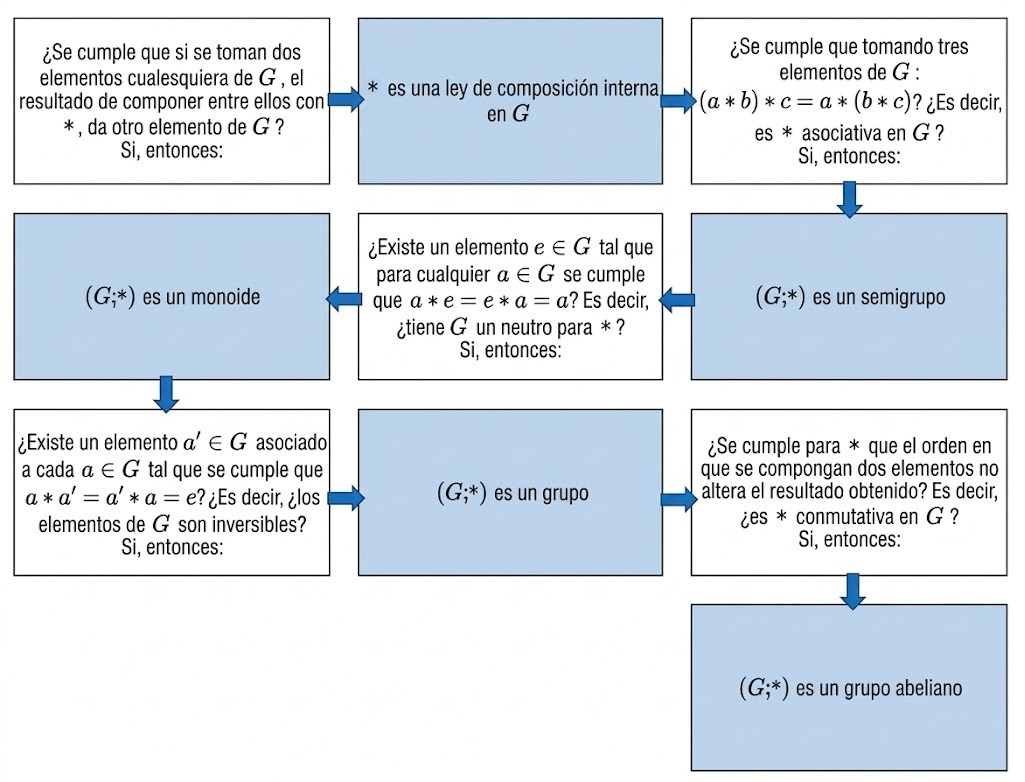
\includegraphics[width=0.8\textwidth]{imagenes/EstructurasAlgebraicas_01.jpg}
    \caption{Estructuras algebraicas con una sola operación interna.}
    \label{fig:estructuras-algebraicas-01}
\end{figure}


\noindent \textit{En la próxima sección se presentan las principales estructuras con dos operaciones internas.}

\subsubsection{Anillo}
\label{sec:anillo}  

Un anillo se define formalmente como una estructura algebraica constituida por un conjunto no vacío, denotado comúnmente como $R$, provisto de dos operaciones binarias o leyes de composición interna, habitualmente denominadas adición ($+$) y multiplicación o producto ($\cdot$). Para que la terna $(R, +, \cdot)$ alcance la categoría matemática de anillo, debe satisfacer rigurosamente un conjunto de axiomas interrelacionados:

\begin{itemize}
    \item Bajo la operación de adición, la estructura $(A, +)$ conforma un \textbf{grupo abeliano}, lo cual exige el cumplimiento de la asociatividad, la conmutatividad, la existencia de un elemento neutro aditivo y de un opuesto aditivo para todos y cada uno de los elementos del conjunto.
    
    \begin{itemize}
        \item \textbf{Asociatividad:} $(a + b) + c = a + (b + c)$ para todo $a, b, c \in R$.
        \item \textbf{Existencia de elemento neutro ($0$):} Existe $0 \in R$ tal que $a + 0 = a$ para todo $a \in R$.
        \item \textbf{Existencia de elemento simétrico (opuesto):} Para cada $a \in R$, existe $-a \in R$ tal que $a + (-a) = 0$.
        \item \textbf{Conmutatividad:} $a + b = b + a$ para todo $a, b \in R$.
    \end{itemize}    
    
    \item Bajo la operación de multiplicación, el sistema $(A, \cdot)$ constituye un \textbf{semigrupo}; es decir, la multiplicación debe ser inexcusablemente asociativa.
    \begin{itemize}
        \item \textbf{Clausura:} Si $a, b \in R$, entonces $a \cdot b \in R$.
        \item \textbf{Asociatividad:} $(a \cdot b) \cdot c = a \cdot (b \cdot c)$ para todo $a, b, c \in R$.
    \end{itemize}

    \item Ambas leyes de composición se vinculan estructuralmente mediante la \textbf{propiedad distributiva} de la multiplicación respecto de la adición, exigiéndose su cumplimiento tanto por la izquierda como por la derecha.    
    \begin{itemize}
        \item \textbf{Distributividad por la izquierda:} $a \cdot (b + c) = (a \cdot b) + (a \cdot c)$.
        \item \textbf{Distributividad por la derecha:} $(b + c) \cdot a = (b \cdot a) + (c \cdot a)$.
    \end{itemize}

\end{itemize}

\textbf{Propiedades algebraicas fundamentales}\\
A partir de su definición fundacional, se deducen propiedades operativas inherentes a cualquier anillo. Por ejemplo:

\begin{itemize}
    \item \textbf{Elemento absorbente:} $a \cdot 0 = 0 \cdot a = 0$.\\
    El elemento neutro de la suma actúa como elemento absorbente para la multiplicación.

    \item \textbf{Regla de los signos:} $a \cdot (-b) = (-a) \cdot b = -(a \cdot b)$ y $(-a) \cdot (-b) = a \cdot b$.\\
    Rigen las reglas algebraicas de los signos.
\end{itemize}

\textbf{Clasificación} \\
La estructura de un anillo admite mayores grados de regularidad al imponerse axiomas 
suplementarios a la multiplicación.\\
\begin{itemize}
    \item \textbf{Anillo Conmutativo:} Si la ley multiplicativa goza de la propiedad conmutativa ($a \cdot b = b \cdot a$). \\
    Ejemplo: $(\mathbb{Z}, +, \cdot)$.
    \item \textbf{Anillo Unitario} o con unidad Si posee un elemento neutro multiplicativo (denotado por$1$). \\
    Siendo $1_R$, tal que $a \cdot 1_R = 1_R \cdot a = a$.\\ 
    Ejemplo: $(\mathbb{Z}, +, \cdot)$.    
    \item \textbf{Anillo de División} Se dice que un elemento es inversible, o una unidad, si admite un simétrico multiplicativo dentro del anillo.  \\
    Siendo ($a^{-1}$) tal que $a \cdot a^{-1} = a^{-1} \cdot a = 1_R$. Un anillo unitario es un anillo de división si cada elemento no nulo es una unidad.\\
    Ejemplo: $(\mathbb{Z}, +, \cdot)$ NO es un anillo de división.
\end{itemize}

Un concepto de profundo calado analítico es la existencia de \textbf{divisores de cero}. En un anillo, dos elementos no nulos $a$ y $b$ son divisores de cero si su producto resulta en el neutro aditivo ($ab = 0$). La ausencia de divisores de cero garantiza la validez de la ley de simplificación. Cuando un anillo conmutativo y unitario carece estrictamente de divisores de cero, se erige como un \textbf{dominio de integridad}.


\subsubsection{Cuerpo}
\label{sec:cuerpo}    
Un cuerpo representa el nivel más alto de regularidad operativa. Si un anillo permite sumar y multiplicar, un cuerpo es, esencialmente, un anillo donde además es posible dividir por cualquier elemento que no sea el cero.

\textbf{Definición Axiomática de Cuerpo}

Sea $K$ un conjunto no vacío dotado de dos leyes de composición interna: suma ($+$) y producto ($\cdot$). La estructura $(K, +, \cdot)$ es un cuerpo si se satisfacen los siguientes tres pilares:

\begin{itemize}
\item \textbf{$(K, +)$ es un Grupo Abeliano} \\
Se cumplen las propiedades de clausura, asociatividad, existencia de elemento neutro ($0$), existencia de elemento opuesto ($-a$) y conmutatividad.

\item \textbf{$(K \setminus \{0\}, \cdot)$ es un Grupo Abeliano} \\
Esta es la condición crítica que diferencia al cuerpo de un anillo común. Para el producto se exige:
\begin{itemize}
    \item \textbf{Clausura:} El producto de dos elementos no nulos es no nulo.
    \item \textbf{Asociatividad:} $(a \cdot b) \cdot c = a \cdot (b \cdot c)$.
    \item \textbf{Existencia de elemento unidad ($1$):} Tal que $a \cdot 1 = a$.
    \item \textbf{Existencia de elemento inverso:} Para cada $a \in K, a \neq 0$, existe $a^{-1} \in K$ tal que $a \cdot a^{-1} = 1$.
    \item \textbf{Conmutatividad:} $a \cdot b = b \cdot a$.
\end{itemize}

\item \textbf{Distribución}
El producto es distributivo respecto a la suma: $a \cdot (b + c) = a \cdot b + a \cdot c$.
\end{itemize}

\textbf{Diferencias Clave con los Anillos}\\
Es importante distinguir por qué no todos los anillos son cuerpos, por ejemplo en el anillo de los enteros $(\mathbb{Z}, +, \cdot)$, el elemento $2$ no tiene un inverso multiplicativo que sea entero ($1/2 \notin \mathbb{Z}$). Por lo tanto, $\mathbb{Z}$ es un anillo, pero no un cuerpo.

 \textbf{Ausencia de Divisores de Cero} \\
 Una de las propiedades más potentes de un cuerpo es que carece de divisores de cero, lo que lo convierte en un dominio de integridad.En un cuerpo ($K$): Si $a \cdot b = 0$, entonces necesariamente $a = 0$ o $b = 0$. Esta propiedad permite la cancelación en ecuaciones ($ax = ay \implies x = y$ para $a \neq 0$).

 Los cuerpos son la base del Álgebra Lineal. Sin la estructura de cuerpo en el conjunto de escalares, no se podrían definir los espacios vectoriales tal como los conocemos, ya que la resolución de sistemas de ecuaciones lineales requiere la existencia de inversos multiplicativos para despejar incógnitas.
 
\subsubsection{Álgebra de Boole}
\label{sec:algebra-de-boole}

Álgebra de Boole es una estructura algebraica $(B, +, \cdot, ', 0, 1)$ donde $B$ es un conjunto no vacío, ( $+$ ) y ( $\cdot$ ) son dos leyes de composición interna (denominadas usualmente suma y producto),( $'$ ) es una operación unaria (complemento), y $0$ y $1$ son elementos singulares (neutros).

Para que la estructura sea considerada un Álgebra de Boole, debe satisfacer los siguientes postulados (basados en los axiomas de Huntington):

\begin{itemize}
    \item \textbf{Clausura:} Para todo $a, b \in B$, tanto $a + b$ como $a \cdot b$ pertenecen a $B$.
    \item \textbf{Propiedad Conmutativa:} 
    \begin{itemize}
        \item $a + b = b + a$
        \item $a \cdot b = b \cdot a$
    \end{itemize}
    \item \textbf{Propiedad Distributiva (Simetría Axiomática):} A diferencia de los anillos comunes, aquí ambas operaciones son distributivas respecto a la otra:
    \begin{itemize}
        \item $a + (b \cdot c) = (a + b) \cdot (a + c)$
        \item $a \cdot (b + c) = (a \cdot b) + (a \cdot c)$
    \end{itemize}
    \item \textbf{Elementos Neutros:} Existen $0, 1 \in B$ tales que:
    \begin{itemize}
        \item $a + 0 = a$
        \item $a \cdot 1 = a$
    \end{itemize}
    \item \textbf{Propiedad del Complemento:} Para cada $a \in B$, existe un único $a' \in B$ tal que:
    \begin{itemize}
        \item $a + a' = 1$
        \item $a \cdot a' = 0$
    \end{itemize}
\end{itemize}



\section{Los Números Enteros}
\label{sec:numeros-enteros}

\subsection{Dominio de Integridad} 
\label{sec:dominio_de_integridad}

a desarrollar ....


\end{document}